\documentclass{report}


\usepackage{amsmath} % Better matrix environment
\usepackage{amssymb}
\usepackage[inline]{enumitem} % inline numbering and resume numbering
\usepackage{etoolbox} % If conditions
\usepackage{graphicx}
\usepackage{listings} % for code
\usepackage{hyperref}
\usepackage{caption}
\usepackage{subcaption}
\usepackage{tikz}
\usepackage{tikz-qtree,tikz-qtree-compat} % Trees
\usepackage{xkeyval}


% Squiggly lines
\usetikzlibrary{decorations.pathmorphing}


% Node shapes
\usetikzlibrary{shapes,decorations}

\newcommand{\VertexSet}{V}
\newcommand{\CellSet}{C}

\newcommand{\Visited}{V_{visited}}

% Adjacency relation
\newcommand{\AdjVV}{Adj_{\VertexSet\VertexSet}}

% Cardinality of
\newcommand{\card}[1]{\left\vert{#1}\right\vert}

% powerset of
\newcommand{\powerset}[1]{\mathcal P \left({#1}\right)}


% Tikz function: compute absolute position
% row, delta-sy, y-offset
\newcommand{\rctoxy}[3][3=0]{#1*#2 + #3}



% Line that can go anywhere, structured region or outside
\tikzset{%
    anywhere/.style={
		decorate,
		decoration={
		    snake,
		    segment length=4,
		    amplitude=.9,post=lineto,
		    post length=2pt
		}
	}
}

% Line that can only go outside the structured region
\tikzset{outside/.style={dotted}}


% Ellipsis
\tikzset{ellipsis/.style={loosely dotted}}

% Structured
\tikzset{structured/.style={}}


%% Node labelling functions

% row, col, rowoffset, coloffset
\newcommand{\plainlabelnode}[4]{
\pgfmathtruncatemacro{\rowlabel}{#1+#3}\pgfmathtruncatemacro{\collabel}{#2+#4}$n_{\rowlabel,\collabel}$}

% row, col, rowoffset, coloffset, column-variable
\newcommand{\varcollabelnode}[5]{
\pgfmathtruncatemacro{\row}{#1+#3}\pgfmathtruncatemacro{\col}{#2+#4}\pgfmathtruncatemacro{\colzero}{\col-1}\newcommand{\collabel}{\ifnumcomp{\colzero}{=}{0}{#5}{\ifnumcomp{\colzero}{>}{0}{#5+\colzero}{#5\colzero}}}$n_{\row,\collabel}$}

% row, col, rowoffset, coloffset, row-variable
\newcommand{\varrowlabelnode}[5]{\pgfmathtruncatemacro{\row}{#1+#3}\pgfmathtruncatemacro{\rowzero}{\row-1}\pgfmathtruncatemacro{\col}{#2+#4}\newcommand{\rowlabel}{\ifnumcomp{\rowzero}{=}{0}{#5}{\ifnumcomp{\rowzero}{>}{0}{#5+\rowzero}{#5\rowzero}}}$n_{\rowlabel,\col}$}


% row, col, rowoffset, coloffset, row-variable, col-variable
\newcommand{\varlabelnode}[6]{\pgfmathtruncatemacro{\row}{#1+#3}\pgfmathtruncatemacro{\rowzero}{\row-1}\pgfmathtruncatemacro{\col}{#2+#4}\pgfmathtruncatemacro{\colzero}{\col-1}\newcommand{\rowlabel}{\ifnumcomp{\rowzero}{=}{0}{#5}{\ifnumcomp{\rowzero}{>}{0}{#5+\rowzero}{#5\rowzero}}}\newcommand{\collabel}{\ifnumcomp{\colzero}{=}{0}{#6}{\ifnumcomp{\colzero}{>}{0}{#6+\colzero}{#6\colzero}}}$n_{\rowlabel,\collabel}$}



\pgfkeys{/tikz/.cd,% to set the path
  rows/.get=\krows,
  rows/.store in=\krows,
  cols/.get=\kcols,
  cols/.store in=\kcols,
  rowoffset/.initial=0,
  rowoffset/.get=\krowoffset,
  rowoffset/.store in=\krowoffset,
  coloffset/.initial=0,
  coloffset/.get=\kcoloffset,
  coloffset/.store in=\kcoloffset,
  labeler/.get=\klabeler,
  labeler/.store in=\klabeler,
  labelerA/.get=\klabelerA,
  labelerA/.store in=\klabelerA,
  labelerB/.get=\klabelerB,
  labelerB/.store in=\klabelerB,
  labelerC/.get=\klabelerC,
  labelerC/.store in=\klabelerC,
  labelerD/.get=\klabelerD,
  labelerD/.store in=\klabelerD,
  northborder/.initial=outside,
  northborder/.get=\knorthborder,
  northborder/.store in=\knorthborder,
  southborder/.initial=outside,
  southborder/.get=\ksouthborder,
  southborder/.store in=\ksouthborder,
  eastborder/.initial=outside,
  eastborder/.get=\keastborder,
  eastborder/.store in=\keastborder,
  westborder/.initial=outside,
  westborder/.get=\kwestborder,
  westborder/.store in=\kwestborder,
}

%% Draws a grid - num rows, num cols, row offset, col offset
\newcommand{\drawgrid}[1]{{
     \tikzset{#1}


	\newcommand{\maxrows}{\krows}
	\newcommand{\maxcols}{\kcols}
	\newcommand{\rowoffset}{\krowoffset}
	\newcommand{\coloffset}{\kcoloffset}
	% Argument is a function: r,c -> node label
	\newcommand{\labeler}{\klabeler}

	\foreach \row in {1,...,\maxrows} {
		\pgfmathsetmacro{\ypos}{-2 * \row + \rowoffset}
		\pgfmathtruncatemacro{\prevrow}{\row - 1}

		\foreach \col in {1,...,\maxcols} {
			\pgfmathsetmacro{\xpos}{2 * \col + \coloffset}
			\pgfmathtruncatemacro{\prevcol}{\col - 1}
			\newcommand{\thisnode}{(n \row \space \col)}

			% Get node label
			\ifstrempty{\klabelerA}{
				\newcommand{\nodelabel}{\labeler{\row}{\col}}
			}
			\ifstrempty{\klabelerB} {
				\newcommand{\nodelabel}{\labeler{\row}{\col}{\klabelerA}}
			}
			\ifstrempty{\klabelerC} {
				\newcommand{\nodelabel}{\labeler{\row}{\col}{\klabelerA}{\klabelerB}}
			}
			\ifstrempty{\klabelerD} {
				\newcommand{\nodelabel}{\labeler{\row}{\col}{\klabelerA}{\klabelerB}{\klabelerC}}
			}
			{
				\newcommand{\nodelabel}{\labeler{\row}{\col}{\klabelerA}{\klabelerB}{\klabelerC}{\klabelerD}}
			}
			% Create node
			\node (n \row \space \col) at (\xpos,\ypos) {\nodelabel};

			% Line from node to the previous horizontal node
			\ifnumcomp{\col}{>}{1} {
				\draw (n \row \space \prevcol) -- \thisnode;
			}

			% Line from node to the previous vertical node
			\ifnumcomp{\row}{>}{1} {
				\draw (n \prevrow \space \col) -- \thisnode;
			}


			% West border lines
			\ifnumcomp{\col}{=}{1} {
				\draw[\kwestborder] \thisnode -- (\xpos-1, \ypos);
			}
			% East border lines
			\ifnumcomp{\col}{=}{\maxcols} {
				\draw[\keastborder] (\xpos+1, \ypos) -- \thisnode;
			}

			% North border lines
			\ifnumcomp{\row}{=}{1} {
				\draw[\knorthborder] \thisnode -- (\xpos, \ypos+1);
			}
			% South border lines
			\ifnumcomp{\row}{=}{\maxrows} {
				\draw[\ksouthborder] (\xpos, \ypos-1) -- \thisnode;
			}
		}
	}
}}
\pgfkeys{/tikz/.cd,% to set the path
  num/.get=\knum,
  num/.store in=\knum,
  rowoffset/.initial=0,
  rowoffset/.get=\krowoffset,
  rowoffset/.store in=\krowoffset,
  coloffset/.initial=0,
  coloffset/.get=\kcoloffset,
  coloffset/.store in=\kcoloffset,
}


%% Draws a row of vertical ellipses - num cols, row offset, col offset
\newcommand{\drawellipsisrow}[1]{{
	\tikzset{#1}

	\newcommand{\numellipses}{\knum}
	\newcommand{\rowoffset}{\krowoffset}
	\newcommand{\coloffset}{\kcoloffset}

	\foreach \col in {1,...,\numellipses} {
		\pgfmathsetmacro{\xpos}{2 * \col + \coloffset}
		\pgfmathsetmacro{\ypos}{\rowoffset}

		\draw[ellipsis] (\xpos, \ypos) -- (\xpos, \ypos-1);
	}
}}



\pgfkeys{/tikz/.cd,% to set the path
  num/.get=\knum,
  num/.store in=\knum,
  rowoffset/.initial=0,
  rowoffset/.get=\krowoffset,
  rowoffset/.store in=\krowoffset,
  coloffset/.initial=0,
  coloffset/.get=\kcoloffset,
  coloffset/.store in=\kcoloffset,
}


%% Draws a column of horizontal ellipses - num rows, row offset, col offset
\newcommand{\drawellipsiscol}[1]{{
	\tikzset{#1}

	\newcommand{\numellipses}{\knum}
	\newcommand{\rowoffset}{\krowoffset}
	\newcommand{\coloffset}{\kcoloffset}

	\foreach \row in {1,...,\numellipses} {
		\pgfmathsetmacro{\xpos}{\coloffset}
		\pgfmathsetmacro{\ypos}{-2 * \row + \rowoffset}

		\draw[ellipsis] (\xpos, \ypos) -- (\xpos+1, \ypos);
	}
}}


\begin{document}

\chapter{Introduction}
Scientific computing is a large research branch touching on various areas in the scientific community as well as in various industries. An integral part of it is concerned with algorithms and techniques which operate on a mesh representation of a model, typically modelling physical phenomena such as the motion of fluids. SEE
% [Flow simulation and high performance computing, 1996a T. Tezduyar, http://www.tafsm.org/PUB_PRE/jALL/j63-CM96.pdf]
. SEE
% [http://www.sv.vt.edu/classes/MSE2094_NoteBook/97ClassProj/num/widas/history.html]
for a good introduction on finite element analysis.


Various methods of representing meshes exist, including X, Y, and Z
% [http://en.wikipedia.org/wiki/Polygon_mesh#Representations]
. Representations typically rely on encoding some form of explicitly-defined mapping between mesh elements. This can be represented straightforwardly as a flat array, with the array indices representing elements in the source set, and each value being one or more values representing one or more elements in the destination/target set. We focus our attention to the case where the number of target elements mapped to from each source element is constant. Such a map is known as a constant-arity map.

Consider for instance a quadrilateral mesh with two element sets \texttt{C} and \texttt{V}, representing the set of cells and vertices, respectively.
We can define a dat of coordinates, which associates the set each vertex $v \in V$ with a coordinate pair $(x_v, y_v)$, representing its position in 2D space.

We can then define an adjacency map (of constant arity 4) from cells to vertices:

\texttt{$C \rightarrow Node^4$}

Now consider an operation over this mesh, which performs a computation for each cell $c \in C$ as a function of its adjacent nodes ${n | n \in Map[c]}$, for instance computing the area of the cell. In particular consider the chain of memory access indirections and the resulting memory access patterns:

%
%             |   |             |   |
%             |   |  /----n3--->|   | -> (x_1, y_1)
%             |   | /           |   |
% cell_id ->  |   |/------n1--->|   | -> (x_4, y_4)
%             |   |\            |   |
%             |   | \-----n4--->|   | -> (x_5, y_5)
%             |   |  \          |   |
%             |   |   \---n2--->|   | -> (x_12, y_12)
%             |   |             |   |
%             |   |             |   |
%             |   |             |   |
%           cell2nodes         node2coordinate

Notice that proximate (or indeed adjacent) nodes in the mesh need not exhibit a uniform memory access pattern. This is detrimental to performance for various reasons.
1. They do not exhibit spatial locality, a property which most modern CPU caches bank on to attain higher performance in IO bound applications, which may manifest through decisions regarding cache replacement strategies or data pre-fetching.
2. Looking up addresses, as opposed to computing them directly, will typically prohibit or limit the scope of compiler-performed optimizations, not least vectorizations.

Numerous strategies have been devoted to deal with this problem, notably applying a space filling curve to obtain a more favourable numbering, with closer elements tending to have closer numberings. While the space filling curve most certainly improves cache locality, it does not make use more obvious structure that may exist. A mesh that is irregular and unstructured on the whole may contain subregions of high regularity and uniform structure, whose regularity/uniformity may be locally exploitable in a more direct manner, for potentially higher gain!


We present Crystal mesh, a group of algorithms for \emph{extracting} regions of regularity in a mesh, reorganizing the mesh to \emph{expose} said structure in order to enable efficient \emph{exploitation}.
In particular, we present and evaluate an implementation for extracting and exposing structure in quadrilateral meshes on various examples, and evaluate a 33\% performance improvement achieved by exploiting the structure on the airfoil computation.


\chapter{Background}
Before continuing further, we introduce briefly the main notions required to appreciate this work.

\section{The mathematical mesh model}

Meshes often model physical objects and phenomena. This is typically achieved through the discretization of a continuous model, such as the surface or volume of an object, in order to approximate its physical properties to a desired degree of precision.
\par

The mesh model consists of a hierarchy of elements, which may include a subset the following:
\begin{itemize}
\item Polyhedra such as cubes or tetrahedrons
\item Polygons \emph{(also referred to as cells or faces)} such as triangles and quadrilaterals
\item Edges
\item Vertices \emph{(also referred to as nodes)}
\end{itemize}

\includesvg[width=\imagewidth, svgpath=images/background/]{mesh-elements}

Each element in the above hierarchy is built-up from those below it. Thus, a polyhedron is assimilated by a set of polygons, a polygon is composed by a set of edges, and an edge joins two vertices.


\subsection{Geometry vs topology}
There is a key distinction to make between the geometric and topological properties of a mesh.

Since meshes model a physical reality, the elements of a mesh may be spatially embedded: vertices are associated with points in space, and edges are formed as segments joining their two vertices. This affects \emph{geometric} properties of the mesh, such as its surface area or volume.

On the other hand, the hierarchy of elements described above induces a mesh topology. This describes the connectedness of the mesh, that is to say how elements relate to one another. For instance, we may describe two vertices sharing an edge as \emph{adjacent}, or two cells being sharing an edge as being \emph{incident} on that edge.
\par
In this work we concern ourselves solely with the topological structure of meshes, treating its geometry as arbitrary data that is associated with its respective elements (the position of a vertex for instance). Figure~\ref{fig:same-topology} illustrates the difference between the two concepts.

\begin{figure}
    \includesvg[width=\imagewidth, svgpath=images/background/]{same-topology}
    \caption{Despite having completely different geometric shapes and properties, the two meshes are topologically equivalent. The labels indicate corresponding vertices.}
    \label{fig:same-topology}
\end{figure}




\subsection{Manifold meshes}
A mesh is a manifold if the following properties hold:
\begin{enumerate}
\item All edges are adjacent to either one or two faces.

\item All faces meeting at a given vertex must form either an open or a closed fan around that vertex (Figure~\ref{fig:open-closed-fans}).
\end{enumerate}

% Open and closed fans
\begin{figure}
    \sidebyside
        {\includesvg[width=\imagewidth, svgpath=images/background/]{closed-fan}
        \caption{A closed fan}}
        {\includesvg[width=\imagewidth, svgpath=images/background/]{open-fan}
        \caption{An open fan}}
    \caption{}
    \label{fig:open-closed-fans}
\end{figure}

Figure~\ref{fig:non-manifolds} demonstrates examples of non-manifold meshes. In this work we consider manifold meshes exclusively, and future mentions of `mesh' shall implicitly refer to manifold meshes.

% Non-manifolds
\begin{figure}
    \sidebysidefour
    {\includesvg[width=\textwidth, svgpath=images/background/]{bad-fan}
        \caption{Faces incident on a vertex which do not form a continuous fan}}
    {\includesvg[width=\textwidth, svgpath=images/background/]{bad-fan2}
        \caption{An extra face that breaks off from the otherwise closed fan}}
    {\includesvg[width=\textwidth, svgpath=images/background/]{bad-multi-edge}
        \caption{More than two faces incident on a single edge}}
    {\includesvg[width=\textwidth, svgpath=images/background/]{bad-no-edge}
        \caption{An edge with no incident faces}}

    \caption{Examples of non-manifold meshes.}
    \label{fig:non-manifolds}
\end{figure}





\section{The mesh data structure}

We describe how a mesh model is manifest at the data structure level. There are three general component types can be identified:
\begin{itemize}
\item Entity sets
\item Associative data
\item Relations between two entity sets
\end{itemize}

In the following sections, the examples shall refer to the mesh depicted in figure~\ref{fig:example-mesh}.

\begin{figure}
    \includesvg[width=\textwidth, svgpath=images/background/]{mesh-data-structure}
    \caption{Example mesh with labelled elements.}
    \label{fig:example-mesh}
\end{figure}


\subsection{Entity sets}
Each set represents a certain type of entity in the mesh, such as vertices or cells. Each element in a set is associated with a unique identifier. Integers are a common choice as an identifier for a couple of reasons:
\begin{itemize}
\item They need not be enumerated explicitly. All we need is the set cardinality and a starting index.
\item They are convenient for direct-indexed array accesses, as well as for more general indexing methods.
\end{itemize}

See figure~\ref{fig:entity-sets} for examples.

\begin{figure}
    \includesvg[width=\textwidth, svgpath=images/background/]{entity-sets}
    \caption{The entity sets of the mesh in figure~\ref{fig:example-mesh}. These are (from left to right) the vertices, edges, and cells.}
    \label{fig:entity-sets}
\end{figure}


\subsection{Associative data}
Arbitrary data which is associated with elements of a particular entity set. For instance, spatial coordinates associated with each vertex. A typical representation is a flat array indexed by element identifier.
This is the data over which we perform our computations and ultimately care about. Everything else is incidental.
See figure~\ref{fig:associative-data} for an example.

\begin{figure}
    \includesvg[width=\textwidth, svgpath=images/background/]{associative-data}
    \caption{Coordinate data associated with the vertices of the mesh in figure~\ref{fig:example-mesh}.}
    \label{fig:associative-data}
\end{figure}


\subsection{Relation maps between two entity sets}
Entity sets may have relations defined between them, a mapping from an element in a source set to one or more corresponding elements in the destination set. For instance, we may have an adjacency relation from the vertex set to itself, or an inclusion relation from the cell set to the vertex set.
In a general unstructured mesh these relations must be explicitly stored, typically as an array indexed by the source element's identifier.
See figure~\ref{fig:relation} for an example.

\begin{figure}
    \includesvg[width=\textwidth, svgpath=images/background/]{relation}
    \caption{Inclusion relation from cells to vertices, as depicted in the mesh of figure~\ref{fig:example-mesh}.}
    \label{fig:relation}
\end{figure}




\section{The core-computation contract}
Given a mesh model and its underlying representation, computation logic provided by an external user is to be executed. We refer to this as the \emph{core-computation} so as to disambiguate it from other incidental processing, such as structure detection.
Our contract to the user is described in what follows.

\subsection{Given: operating set}
We are given an entity set over which to operate, for example the set of edges or the set of cells. We refer to this entity set as the \emph{operating set}. The core-computation consists of executing a computation for each element of the operating set. This is analogous to the \emph{map} phase of the MapReduce programming model~\cite{dean2008mapreduce}, though we restrict our usage of the term \emph{map} to refer to relation maps.

\subsection{Given: relation-map tree}
We are given a tree structure defining which relation maps to use and how to access them. This is best explained through an example, illustrated in figure~\ref{fig:relation-tree}. The core-computation will, for each element in the operating set, gather all indexing variables as described by the relation-map tree.


\begin{figure}
    %% Key icon
    \newcommand{\keyicon}{\includesvg[width=6pt, svgpath=images/background/]{key}}

    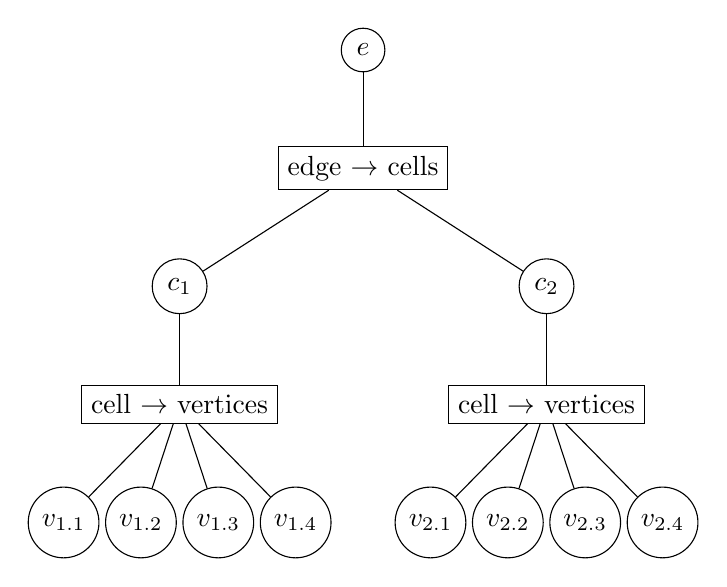
\begin{tikzpicture}[every tree node/.style={draw,circle},
        level distance=1.5cm,
        edge from parent path={(\tikzparentnode) -- (\tikzchildnode)}]

    \tikzset{level 2/.style={sibling distance=0.8cm}}

    \Tree
    [.{$e$}
        \edge node[auto=right] {\keyicon};
        [.\node[rectangle] {edge $\rightarrow$ cells};
            [.{$c_1$}
                \edge node[auto=right] {\keyicon};
                [.\node[rectangle] {cell $\rightarrow$ vertices};
                    [.$v_{1.1}$ ]
                    [.$v_{1.2}$ ]
                    [.$v_{1.3}$ ]
                    [.$v_{1.4}$ ]
                ]
            ]
            [.{$c_2$}
                \edge node[auto=right] {\keyicon};
                [.\node[rectangle] {cell $\rightarrow$ vertices};
                    [.$v_{2.1}$ ]
                    [.$v_{2.2}$ ]
                    [.$v_{2.3}$ ]
                    [.$v_{2.4}$ ]
                ]
            ]
        ]
    ]
    \end{tikzpicture}
    \caption{
    In this example, we consider a core-computation operating over the edge set, with $e$ being the indexing variable into the edge set.
    The edge $\rightarrow$ cells map is indexed by $e$ to obtain the the two cells $c_1$ and $c_2$ incident on the edge $e$. The cell $\rightarrow$ vertices map is then indexed by both $c_1$ and $c_2$ to obtain their respective vertices. The key symbol denotes indexing into the map below, using the indexing variable above.
    }
    \label{fig:relation-tree}
\end{figure}


\subsection{Given: kernel function}
\label{subsec:given-kernel-function}
We are given a kernel function specifying the computation logic, which is applied to each element in the operating set. It takes as arguments all gathered indexing variables, including that of the current element, and it has read and write access to the mesh's associated data. The access pattern of a kernel function is similar to that of a stencil computation, as defined by~\cite{tang2011pochoir}:
\begin{quote}
A stencil computation repeatedly updates each point of a d-dimensional grid as a function of itself and its near neighbours.
\end{quote}
As we define it, however, kernel functions are in fact more general than a stencil computation, as they access neighbouring elements across different operating sets.


The kernel function is applied to the operating set elements in no particular order; the indexing variables, however, are passed to the kernel in some known order, typically in the order stored in the relation-map.


\subsection{Expected operation}
Given all the above, a core-computation is then performed as follows:
\begin{enumerate}
\item Iterate over the elements of the operating set, in no particular order.
\item For each element iterated over:
    \begin{enumerate}
    \item Gather any indexing variables as defined by the relation-map tree. This may involve indexing variables obtained through a chain of relation-maps.
    \item Call the kernel function, passing the gathered indexing variables in some known order. The kernel function may access any associative data using these indexing variables.
    \end{enumerate}
\end{enumerate}



\section{Background on airfoils}
%% TODO CROSS REFERNCE to benchmarks
While not strictly needed for understanding our work, we nonetheless describe briefly airfoils and their function to offer a broader context. Much of this section was adapted from~\cite{abbott2012theory}, \cite{kuethe1986foundations} and~\cite{boeing2014airfoil}. Our description is nonetheless undoubtedly an overly simplistic one, and we would recommend that the aforementioned literature be sought for a fuller picture.

An airplane achieves flight by creating a lower air pressure over the wing (\emph{the upper surface}) whilst maintaining a higher air pressure below the wing (\emph{the lower surface}). The exact way in which this is achieved is characteristic of the wing shape as well as other factors. The pressure differential causes air in the lower surface to push towards the upper surface, creating a lift force. If the lift force is sufficient to counteract the gravitational force, the airplane flies.

An airfoil is the two-dimensional cross-section \emph{shape} of a wing. They are used to model the hydrodynamics (fluid motion) surrounding a particular wing shape in different contexts, including the velocity and angle of motion (known as the \emph{angle of attack}). Figure~\ref{fig:airfoil-crosscut} shows how the cross-section is taken, as well as the modelled air flow.

\begin{figure}
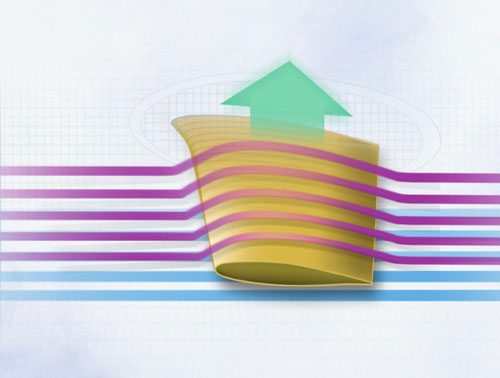
\includegraphics[width=\imagewidth]{images/background/airfoil_crosscut.jpg}
    \caption{The cross-section used to obtain the airfoil shape. Incoming air flow is split between the upper surface (purple) and the lower surface (blue). The image was obtained from~\cite{boeing2014airfoil}.}
    \label{fig:airfoil-crosscut}
\end{figure}


In 1929, the National Advisory Committee for Aeronautics (NACA) began to study various airfoils. They developed families of airfoil constructions parametrized by various geometric variables, depicted in figure~\ref{fig:airfoil-geometry}. We use specific instantiations of these airfoil families as benchmarks for Crystal.

\begin{figure}
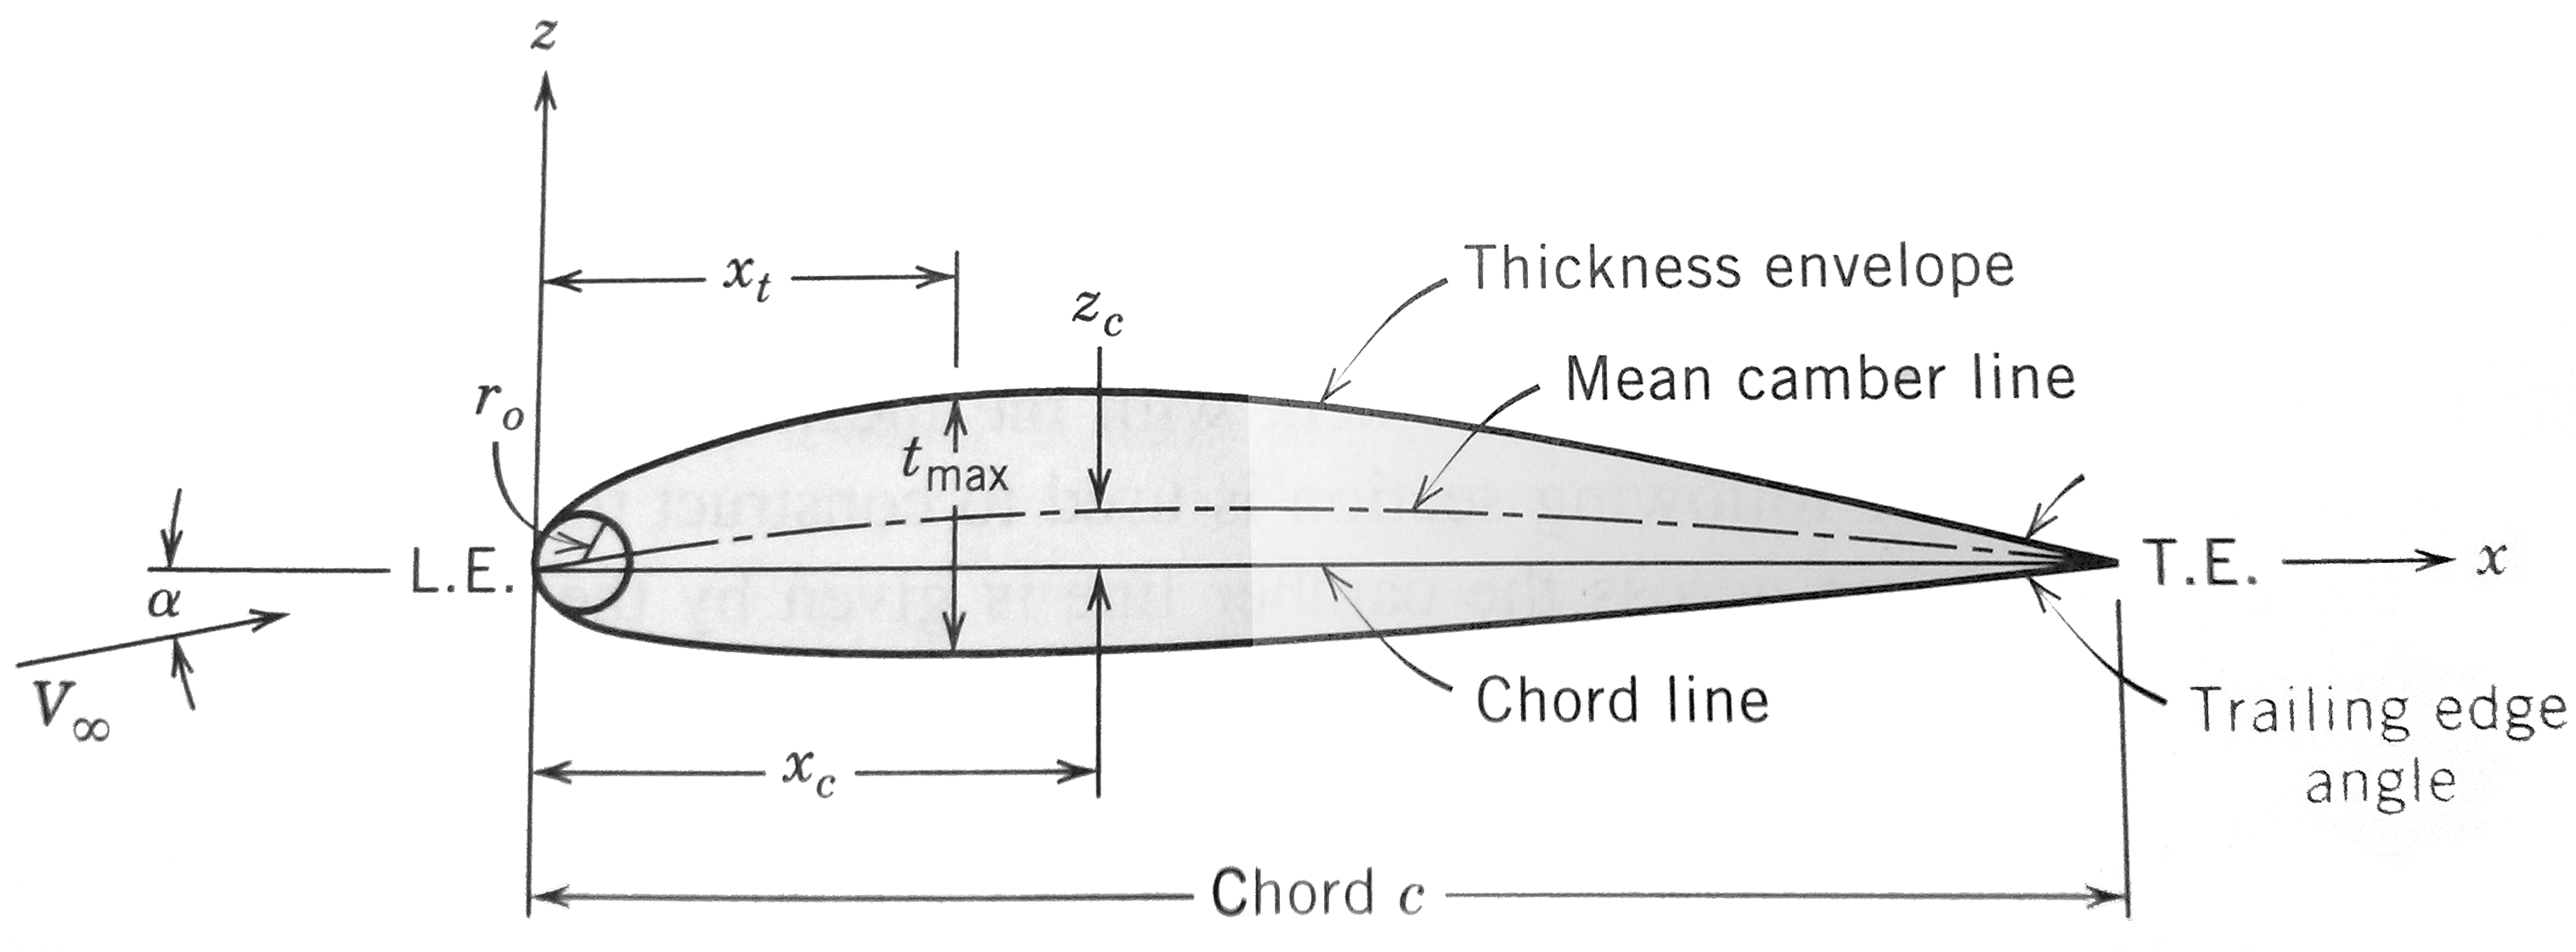
\includegraphics[width=\imagewidth]{images/background/airfoil.png}
    \caption{A depiction of the geometric properties of airfoil. The image was obtained from~\cite{kuethe1986foundations}.}
    \label{fig:airfoil-geometry}
\end{figure}

\section{Chapter summary}
In this chapter we gave a basic description of a mesh as a mathematical model. In addition we defined the concept of the mesh a data structure and how it is used in computation. Finally, we explained the significance of the airfoil in order to have a framing context for our running example.

\chapter{Diving into the problem}
\label{chap:diving-into-problem}
We begin by walking through an example mesh and examining the properties of the structure found within.

\section{A basic definition of structure}
What we would like is a form of structure which is
\begin{enumerate*}[label=\alph*)]
\item representable as a data structure, and \item efficient in terms of performance.
\end{enumerate*}

Given our semantic knowledge about the mesh model we can ascertain some facts about relation-maps:
\begin{itemize}
\item They are sparse: element arity is very small compared to the number of elements, and is in fact unrelated to it.
\item They have a high clustering coefficient: Relationships tend to be localized, forming tightly connected clusters.
% TODO REFERENCE TO CLUSTERING COEFFICIENTS
\end{itemize}

These properties arise as a consequence of meshes modelling real-world phenomena that exist in a Cartesian space.
On this basis, we consider a spatial embodiment of element relationships, organising the elements in a discrete space such that the uniform relationship is apparent.

Bear in mind that this approach carries no relation to any geometric data associated with elements, such as the coordinates of vertices. To make this distinction clear, as well as to emphasize its discrete nature, we address this Cartesian-like space by rows and columns rather than x and y coordinates.

\subsection{Example: Naca0012 mesh}
Figure~\ref{fig:naca12-plain} shows a small extract from the NACA0012 mesh\footnote{Thanks to Dr. Peter Vincent, George Ntemos and Harry Davis}, showing the cross section of an airfoil mesh and its interaction with surrounding fluid. The mesh is discretization into quadrilateral cells over which computations are performed.

\newcommand{\drawnaca}[4]{
	\begin{figure}
	\includesvg[svgpath=#1]{#2}
	\caption{#3}
	\label{#4}
	\end{figure}
}
\drawnaca{images/defining-structure/}{naca0012-plain}{Extract of the NACA0012 mesh.}{fig:naca12-plain}

The vertices in the highlighted region of figure~\ref{fig:naca12-vertices} seem like good candidates for a \emph{``structured region''}, forming a two-dimensional lattice in a discrete Cartesian space. This \emph{``structured region''} has the properties outlined below.

\drawnaca{images/defining-structure/}{naca0012-node-structure}{Highlighted vertices which exhibit a form of \emph{``structured region''}.}{fig:naca12-vertices}

\subsection{Desired properties of a structured region}
\label{sec:structured-region-properties}
\begin{enumerate}
\item All vertices have a uniform arity of four.
\item Every vertex has a consistent discrete direction (for example the cardinal directions: north east, south, west) with respect to the other vertices. In other words, the direction is transitive: if vertex $a$ is above vertex $b$, and vertex $b$ is above vertex $c$, then vertex $a$ is above vertex $c$. For a non-example see figure~\ref{fig:non-consistent-direction}.
\end{enumerate}

\begin{figure}
\includesvg[width=\imagewidth, svgpath=images/defining-structure/]{non-consistent-direction}
\caption{An example of inconsistent direction. We can traverse cells in \emph{``one direction''} by following the edge parallel to the one we entered from. If we start from $A$ and traverse the cells in one direction (the blue path) we reach $Z$. If we start from $A$ and traverse the cells in an orthogonal direction (the red path) to the first path, we also reach $Z$! Is $Z$ then \emph{``above''} $A$ or \emph{``to the side of it''}?}
\label{fig:non-consistent-direction}
\end{figure}


%% TODO Maybe not introduce data structure yet????
We can propagate this inherent structure from the mesh model to the underlying data structure, representing this two-dimensional lattice using a two-dimensional array. Vertices may be assigned Cartesian coordinates, but in spirit of the space's discreteness we shall use rows and columns instead. See figure~\ref{fig:naca12-structure-grid}.\label{sentence:2d-array}

\drawnaca{images/defining-structure/}{naca0012-node-grid}{The overlaid grid shows the lattice structure more clearly.}{fig:naca12-structure-grid}


\newcommand{\strV}{V_{str}}
\newcommand{\adjstrV}{V_{adjstr}}
\newcommand{\AdjVVstr}{Adj_{\adjstrV\strV}}

Let us call $\VertexSet$ the set of all vertices, and $\strV \subseteq \VertexSet$ the set of vertices in the \emph{``structured region''}.

\subsection{Representing the vertex-vertex adjacency}

Now consider the vertex-vertex adjacency relation $\AdjVV: \VertexSet \mapsto \VertexSet$ in context of the \emph{``structured region''} $\strV$. We can directly locate a particular neighbour of any vertex, for example its north neighbour, so long as that neighbour is also within the structured region. This restricts the set of vertices with fully-accessible neighbours to those which are not on the borders or the fringe of the \emph{``structured region''}. This is the subset of vertices $\adjstrV \subseteq \strV$ which are structured \emph{with respect to} $\AdjVV$. This induces a new relation which operates purely within the structured region:
$$\AdjVVstr: \adjstrV \mapsto \strV$$

Figures~\ref{fig:naca12-structured-highlighted} and~\ref{fig:structure-as-graph} illustrate these two sets.
\drawnaca{images/defining-structure/}{naca0012-node-neighbours}{The interior structured vertices (those not on the fringe) are highlighted in dark blue.}{fig:naca12-structured-highlighted}


\begin{figure}
% Draw structured node region
\begin{tikzpicture}[scale=0.7]
	\newcommand{\stylewithfill}[1]{\tikzstyle{every node}=[draw, shape=circle, minimum size=0.8cm, fill=#1];}
	\stylewithfill{none}

	% ROW 0
	\drawgrid{rows=1, cols=3, rowoffset=0, coloffset=4, labeler=\plainlabelnode, labelerA=0, labelerB=2,
		southborder=structured}

	% ROW 1
	\drawgrid{rows=1, cols=2, rowoffset=-2, coloffset=0, labeler=\plainlabelnode, labelerA=1, labelerB=0,
		eastborder=structured}

	{
	\stylewithfill{neighbourstructurecolor}
	\drawgrid{rows=1, cols=2, rowoffset=-2, coloffset=4, labeler=\plainlabelnode, labelerA=1, labelerB=2,
		northborder=structured, southborder=structured, westborder=structured, eastborder=structured}
	}

	\drawgrid{rows=1, cols=1, rowoffset=-2, coloffset=8, labeler=\plainlabelnode, labelerA=1, labelerB=4,
		northborder=structured, southborder=structured, westborder=structured}


	\drawgrid{rows=1, cols=1, rowoffset=-2, coloffset=12, labeler=\plainlabelnode, labelerA=1, labelerB=6,
		southborder=structured, eastborder=structured}

	\drawgrid{rows=1, cols=1, rowoffset=-2, coloffset=14, labeler=\plainlabelnode, labelerA=1, labelerB=7,
		westborder=structured}

	% ROW 2
	\drawgrid{rows=1, cols=1, rowoffset=-4, coloffset=4, labeler=\plainlabelnode, labelerA=2, labelerB=2,
		northborder=structured, southborder=structured, eastborder=structured}

	{
	\stylewithfill{neighbourstructurecolor}
	\drawgrid{rows=1, cols=2, rowoffset=-4, coloffset=6, labeler=\plainlabelnode, labelerA=2, labelerB=3,
		northborder=structured, southborder=structured, eastborder=structured, westborder=structured}
	}

	\drawgrid{rows=1, cols=1, rowoffset=-4, coloffset=10, labeler=\plainlabelnode, labelerA=2, labelerB=5,
		southborder=structured, westborder=structured, eastborder=structured}

	\drawgrid{rows=1, cols=1, rowoffset=-4, coloffset=12, labeler=\plainlabelnode, labelerA=2, labelerB=6,
		northborder=structured, westborder=structured}

	% ROW 3
	\drawgrid{rows=1, cols=1, rowoffset=-6, coloffset=4, labeler=\plainlabelnode, labelerA=3, labelerB=2,
		northborder=structured, southborder=structured, eastborder=structured}

	{
	\stylewithfill{neighbourstructurecolor}
	\drawgrid{rows=1, cols=2, rowoffset=-6, coloffset=6, labeler=\plainlabelnode, labelerA=3, labelerB=3,
		northborder=structured, southborder=structured, eastborder=structured, westborder=structured}
	}

	\drawgrid{rows=1, cols=1, rowoffset=-6, coloffset=10, labeler=\plainlabelnode, labelerA=3, labelerB=5,
		northborder=structured, westborder=structured}

	% ROW 4
	\drawgrid{rows=1, cols=1, rowoffset=-8, coloffset=2, labeler=\plainlabelnode, labelerA=4, labelerB=1, eastborder=structured}

	{
	\stylewithfill{neighbourstructurecolor}
	\drawgrid{rows=1, cols=2, rowoffset=-8, coloffset=4, labeler=\plainlabelnode, labelerA=4, labelerB=2,
		northborder=structured, southborder=structured, eastborder=structured, westborder=structured}
	}

	\drawgrid{rows=1, cols=1, rowoffset=-8, coloffset=8, labeler=\plainlabelnode, labelerA=4, labelerB=4,
		northborder=structured, westborder=structured}

	% ROW 5
	\drawgrid{rows=1, cols=2, rowoffset=-10, coloffset=4, labeler=\plainlabelnode, labelerA=5, labelerB=2,
		northborder=structured}
\end{tikzpicture}
\caption{The vertices in figure~\ref{fig:naca12-structured-highlighted} represented as a graph.}
\label{fig:structure-as-graph}
\end{figure}

The key insight we make is that for structured regions in a mesh we need not represent set relationship maps explicitly; the uniformity of set relations allows us to deduce the relationships. We can encode the relation $\AdjVVstr$ very simply. Given a vertex $n_{r,c} \in \adjstrV$, located at row $r$ and column $c$, its four vertex neighbours are $n_{r,c-1}$, $n_{r,c+1}$, $n_{r-1,c}$, and $n_{r+1,c}$. This is illustrated in figure~\ref{fig:single-vertex-neighbours}.



\begin{figure}
% Draw structured node region
\begin{tikzpicture}[scale=1]
	\newcommand{\stylewithfill}[1]{\tikzstyle{every node}=[draw, shape=circle, minimum size=1.3cm, fill=#1];}
	\stylewithfill{none}

	% ROW 0
	\drawgrid{rows=1, cols=1, rowoffset=0, coloffset=2,
		labeler=\varlabelnode, labelerA=-1, labelerB=0, labelerC=r, labelerD=c,
		southborder=structured}

	% ROW 1
	\drawgrid{rows=1, cols=1, rowoffset=-2, coloffset=0,
		labeler=\varlabelnode, labelerA=0, labelerB=-1, labelerC=r, labelerD=c,
		eastborder=structured}

	{
		\stylewithfill{neighbourstructurecolor}
		\drawgrid{rows=1, cols=1, rowoffset=-2, coloffset=2,
			labeler=\varlabelnode, labelerA=0, labelerB=0, labelerC=r, labelerD=c,
			eastborder=structured, westborder=structured, northborder=structured, southborder=structured}
	}

	\drawgrid{rows=1, cols=1, rowoffset=-2, coloffset=4,
		labeler=\varlabelnode, labelerA=0, labelerB=1, labelerC=r, labelerD=c,
		westborder=structured}

	% ROW 2
	\drawgrid{rows=1, cols=1, rowoffset=-4, coloffset=2,
		labeler=\varlabelnode, labelerA=1, labelerB=0, labelerC=r, labelerD=c,
		northborder=structured}

\end{tikzpicture}
\caption{The neighbours of a structured vertex.}
\label{fig:single-vertex-neighbours}
\end{figure}


\section{Mesh structure as a data structure}
The choice of data structure to represent the structured region is a key one, touching on various aspects:
\begin{itemize}
\item Scope of structure representation: what level of structure can be represented.
\item Implementation complexity of structure detection: how complex a detection algorithm is required.
\item Runtime performance of structure detection: the time and space complexity of the detection algorithm.
\item Storage requirements for detected structure: the storage requirements for the detected structure.
\item Runtime performance of computation over the structured region.
\end{itemize}

We analyse several possible data structure representations.

\subsection{Structure bit-mask}
\label{subsec:structure-bitmap}

\newcommand{\drawbitmap}[2]{
	% trim left bottom right top
	\includesvg[svgpath=#1]{#2}
}

Represent the bounding box around the structured region as a two-dimensional bit-mask, with each bit representing a vertex position in the superimposed grid. An \emph{on} bit indicates that the corresponding vertex is part of the structured region, an \emph{off} bit otherwise.

A bit-mask can represent \emph{any} structured region which adheres to the properties listed in section~\ref{sec:structured-region-properties}. They are very flexible, capable of representing complex formations as well as handling small anomalies in structure.

Let us define the \emph{efficiency} $\epsilon$ of a bit-mask as the percentage of its bits which are \emph{on}, as the \emph{off} bits represent wasted vertices. Bit-masks with high $\epsilon$ are favourable for several reasons:
\begin{itemize}
\item \emph{Off} bits increase the storage space of the structured region, up to $O(\card{\VertexSet})$ in the worst case, as opposed to $O(\card{\Structured})$.
\item \emph{Off} bits similarly worsen the runtime performance, again up to $O(\card{\VertexSet})$ due to wasted execution.
\end{itemize}

Figure~\ref{fig:example-bitmask} shows an example of a good bit-mask candidate.

\begin{figure}
\pgfplotstableread{
	1 1 1 1 1 1
	1 2 2 1 1 1
	1 1 2 1 1 2
	1 1 1 1 1 1
	1 1 1 1 1 2
	2 1 1 1 1 1
}{\bitmapmatrix}
\drawmatrix[cell wd=0.8, cell ht=0.8]{\bitmapmatrix}
\caption{An example of a structured region which can be bit-mask defined. The dotted regions indicate unstructured cells. The blue cells are structured cells. Its efficiency $\epsilon$ is $\frac{30}{36} \approx 83\%$.}
\label{fig:example-bitmask}
\end{figure}

A detection algorithm would likely be implemented using a variant of a general graph search algorithm such as breadth-first search or depth-first search. Further consolidation work may be needed to compact disconnected structured components in order to maximize $\epsilon$. The potential benefits of compaction are illustrated in figure~\ref{fig:disjoint-matrix}.

\begin{figure}
\pgfplotstableread{
	2 2 2 2 2 1
	1 2 2 2 2 1
	1 1 2 2 2 2
	2 1 2 2 2 2
	2 1 2 1 2 2
	2 1 1 1 2 2
}{\disjointAmatrix}
\pgfplotstableread{
	1 2 2 1
	1 1 2 1
	2 1 2 2
	2 1 2 1
	2 1 1 1
}{\disjointBmatrix}

\sidebyside
{
\drawmatrix[cell wd=0.8, cell ht=0.8]{\disjointAmatrix}
\caption{Originally detected structured components.}
\label{subfig:original-components}
}
{
\drawmatrix[cell wd=0.8, cell ht=0.8]{\disjointBmatrix}
\caption{Compacted structured components.}
\label{subfig:compacted-components}
}
\caption{A demonstration of the benefits of disconnect structured components compaction. The detected structured cell components in~\ref{subfig:original-components} are unnecessarily sparse and occupy more space than necessary. After compaction in~\ref{subfig:compacted-components} the space is used is reduced by over 40\%.}
\label{fig:disjoint-matrix}
\end{figure}


\subsection{Row-specific boundaries}

Represent the structured region as a sequence of consecutive fixed-length rows, permitting vertices outside the structured region to cluster at the beginning and ends of each row. A structured region is then represented by the row-length, as well as individual begin and end offsets for each row. This is exemplified in figure~\ref{fig:row-specific}.

\begin{figure}
\pgfplotstableread{
	0 2 1 1 1 1
	2 2 1 1 1 2
	1 1 1 1 2 0
	2 1 1 1 1 1
	1 1 1 1 1 1
	2 2 1 1 2 2
}{\bitmapmatrix}
\drawmatrix[cell wd=0.8, cell ht=0.8]{\bitmapmatrix}
\caption{An example of a structured region which can be represented using row-specific boundaries. Note the white cells, which represent unused structured regions near the boundaries.}
\label{fig:row-specific}
\end{figure}

Storing row-specific boundaries reduces the storage requirement by the order of row-length times.
No executions are wasted as the loop iterations are constrained to vertices in the structured region.
A detection algorithm can be implemented as a simple row-by-row traversal in linear time and space.


On the downside, this scheme trades some of the flexibility offered by the bit-mask representation, in particularly anomalies in structure which do not occur at the boundaries.


\subsection{Full rectangle}

Represent the structured region as a rectangle of given length and width, with all elements corresponding strictly to vertices within the structured region. The structured region is thus simply represented by the length and the width: the number of rows and the number of columns. Figure~\ref{fig:rectangle} shows an example of a rectangle-representable structured region.

The storage requirement is now constant with respect to the size of the structured region.
Loop iterations are fixed for each region, enabling further optimisation opportunities.
A detection algorithm, as above, can be implemented as a simple row-by-row traversal.

On the downside, the scope of structure representable is limited, being only capable of representing rectangles proper. Nonetheless, we stick with detecting rectangular structured regions for the remainder of this work as it seems to be the most promising choice.

\begin{figure}
\pgfplotstableread{
	0 2 2 0 2 0
	2 2 1 1 2 2
	2 0 1 1 2 2
	2 2 1 1 0 0
	0 2 1 1 2 2
	2 2 1 1 2 2
}{\bitmapmatrix}
\drawmatrix[cell wd=0.8, cell ht=0.8]{\bitmapmatrix}
\caption{An example of a rectangular structured region. Note the abundance of unused structured cells.}
\label{fig:rectangle}
\end{figure}

\section{Chapter summary}
In this chapter we derived intuitive definitions structure in a mesh in light of an excerpt from an airfoil mesh. We also discussed different representations in which they can be manifested, and the advantages and disadvantages of each.


\chapter{Rectangle growth strategy}
This chapter covers the detection of rectangular structured regions.

An abstract discussion of various properties of algorithms is presented, and the desirable traits brought forth by each.
Then, a selection of concrete algorithms are described, and their merits and weaknesses examined.


\section{Key concepts}
An \emph{absolute structured position} refers to the position of a structured element with respect to the boundaries of its structured region.
A \emph{relative structured position} refers to the position of a structured element with respect to other structured elements within its structured region. Figure~\ref{fig:structured-position} shows this through an example.


%% Relative vs absolute
\begin{figure}
\newcommand{\nodesize}{1.2}
\newcommand{\rows}{4}
\newcommand{\cols}{4}
\newcommand{\rowsize}{\rows*\nodesize}
\newcommand{\colsize}{\cols*\nodesize+2*0.1}

% Node at position r, c, label
\newcommand{\nodeat}[3]{
	\pgfmathsetmacro{\lerow}{ (\rows - #1) * \nodesize - (\nodesize / 2) - 0.1}
	\pgfmathsetmacro{\lecol}{ (#2 * \nodesize) + (\nodesize / 2) + 0.1}
	\node at (\lecol, \lerow) {#3}
}

\sidebyside
{
	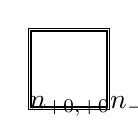
\begin{tikzpicture}
		\tikzstyle{every node}=[draw, shape=rectangle, minimum size=\nodesize cm, font=\small];
		\draw[double] (0,0) rectangle (\colsize,\rowsize);
		\nodeat{2}{1} {$n_{+0,+0}$};
		\nodeat{1}{1} {$n_{-1,+0}$};
		\nodeat{2}{2} {$n_{+0,+1}$};
	\end{tikzpicture}
	\caption{Relative structured position\label{fig:relative-structured-position}}
}
{
	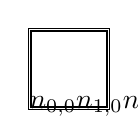
\begin{tikzpicture}
		\tikzstyle{every node}=[draw, shape=rectangle, minimum size=\nodesize cm, font=\small];
		\draw[double] (0,0) rectangle (\colsize,\rowsize);
		\nodeat{0}{0} {$n_{0,0}$};
		\nodeat{1}{0} {$n_{1,0}$};
		\nodeat{0}{1} {$n_{0,1}$};
	\end{tikzpicture}
	\caption{Absolute structured position\label{fig:absolute-structured-position}}
}
\caption{Depiction of \emph{relative} structured position versus \emph{absolute} structured position. The row and column counts are increasing down and to the right, respectively. The borders indicate structured regions, whose origin resides in the top-left corner.\label{fig:structured-position}}
\end{figure}



\section{Properties of detection algorithm}

\subsection{Eager detection}
An eager (or greedy) detection algorithm will include every structured element if finds immediately, regardless of the long term consequences. While this strategy may lead to suboptimal results, it avoids backtracking the structure detection which may be prohibitively costly. Figure~\ref{fig:eager-detection} depicts the sub-optimality of eager detection in contrast with non-eager detection.


\begin{figure}
\pgfplotstableread{
	2 2 2 2 2 2 0
	2 2 1 2 2 0 0
	0 0 1 0 0 0 0
	0 0 1 0 0 0 0
}{\eagermatrix}
\pgfplotstableread{
	2 2 2 2 2 2 0
	2 2 0 2 2 0 0
	1 1 1 1 1 1 1
	1 1 1 1 1 1 1
}{\noneagermatrix}

\sidebyside
{
	\drawmatrix[cell wd=0.6, cell ht=0.6]{\eagermatrix}
	\caption{Eager detection may greedily add the northern cell, yielding a suboptimal structured region.}
}
{
	\drawmatrix[cell wd=0.6, cell ht=0.6]{\noneagermatrix}
	\caption{A non-eager algorithm could instead decide to ignore the northern cell, yielding a larger structured region.}
}
\caption{Eager versus non-eager detection. Black cells and white cells denote unstructured and structured elements, respectively. Red cells denote structured elements detected as forming a rectangular structured region.\label{fig:eager-detection}}
\end{figure}



\subsection{Contiguous detection}
\label{subsec:contiguous-detection}
An algorithm which exhibits continuous detection always adds a structured element which is contiguous to the structured region thus far. The implication is that the relative structured position is always known. This greatly simplifies detection, as all adjacent structured elements are known at any point in time, and structured elements need not be repositioned in the structured region. Figure~\ref{fig:contiguous-detection} contrasts contiguous detection with non-contiguous detection.

In the case of non-contiguous detection, any non-contiguous blobs need to be consolidated. These blobs may be one of three cases:
\begin{enumerate}
\item Disjoint
These may simply be taken as two separate structured regions.

\item Compatible
The blobs can be merged in a lossless manner to form a single structured region.

\item Incompatible
The blobs cannot be merged without loss of structure due to inconsistencies between the blobs. It is then necessary to discard some structured elements.
\end{enumerate}

Examples of the three cases are shown in figure~\ref{fig:non-contiguous-detection}.


% Contiguous versus non-contiguous
\begin{figure}
\pgfplotstableread{
	0 1 1 1 0 0 0 0 0
	0 1 1 1 1 0 0 0 0
	0 1 1 1 0 0 0 0 0
	0 0 1 0 0 0 0 0 0
	0 0 0 0 0 0 0 0 0
}{\contiguousmatrix}
\pgfplotstableread{
	0 1 1 1 0 0 0 0 0
	0 1 1 1 1 0 0 1 0
	0 1 1 1 0 0 1 1 0
	0 0 1 0 0 0 0 0 0
	0 0 0 0 0 0 0 0 0
}{\noncontiguousmatrix}

\sidebyside
{
	\drawmatrix[cell wd=0.6, cell ht=0.6]{\contiguousmatrix}
	\caption{Contiguous detection always adds cells adjacent to the structured region detected thus far.}
}
{
	\drawmatrix[cell wd=0.6, cell ht=0.6]{\noncontiguousmatrix}
	\caption{Non-contiguous detection may add cells which do not border the structured region detected thus far.}
}
\caption{Contiguous detection versus non-contiguous detection algorithms. White cells denote structured elements which have not been added to the structured region. Red cells denote structured elements detected thus far.\label{fig:contiguous-detection}}
\end{figure}

% Types of non-contiguous
\begin{figure}
\sidebysidethreevertical
{
	\includesvg[svgpath=images/detection-algorithms/,width=60mm]{disjoint-blobs}
	\caption{Disjoint blobs of structured elements.}
}
{
	\includesvg[svgpath=images/detection-algorithms/,width=60mm]{compatible-blobs}
	\caption{Compatible blobs of structured elements.}
}
{
	\includesvg[svgpath=images/detection-algorithms/,width=60mm]{incompatible-blobs}
	\caption{Incompatible blobs of structured elements. The two dashed cells are not adjacent in the mesh, but if added as structured element they would have adjacent positions in the structured region.}
}
\caption{Cases that may arise with non-contiguous detection.\label{fig:non-contiguous-detection}}
\end{figure}


\subsection{Post processing requirements}
Different algorithms will require different levels of post-processing in order to yield a rectangular structured region. Some may require a simple operation, such as trimming incomplete rows, while others may require more complex operations to achieve this goal.


\subsection{Detection traversal patterns}
The order in which structured elements are detected in a structured region is important; it imposes some constraints on the data structure representing it. Given the dimensions of the structured region, and knowledge of the absolute structured positions of elements as they are discovered, a simple 2D array allocation would suffice. Any detection order, as is convenient, may be used in this case. However, neither of those facts are known a priori in general.

Various detection traversals orders and their merits are discussed below. Figure~\ref{fig:detection-traversal-patterns} outlines some examples.

\subsubsection{Single-row append-only}
\label{append-detection}
The structured region is grown in a constant direction, for example a single row of structured elements, appended to consecutively. This can be implemented efficiently using either a singly-linked list or a dynamic array with amortized constant time append operation.

\subsubsection{Single-row append/prepend}
\label{append-prepend-detection}
The structured region is grown in either of two directions, for example a single row of structured elements, appended and prepended to. This can be implemented efficiently using a double-ended queue with amortized constant time append and prepend operations.

\subsubsection{Row-oriented detection}
The structured region is represented as a group of rows, with the elements in individual rows grown using one of the above methods. The order in which the rows themselves are grown may also be utilize the same methods, with a nested data structure being a suitable implementation. For example, if rows are detected in an append-only fashion, and the individual elements are detected using append and prepend operations, then a suitable data structure would be a singly-linked list of double-ended queues.

\subsubsection{Indeterminate order detection}
The structured region is grown in a non-linear order: grown elements may not always be contiguous to the structured region thus far. If the growth is indeed non-contiguous, the relative structured positions are \emph{not} always known, and structured elements may need to be repositioned. A possible implementation would be a jagged 2D array, that is an array of arrays, which is expanded as needed. A flat-array-based 2D array would (in the worst case) require reallocating all elements upon expansion, as opposed to reallocating a single row in the case of a jagged 2D array.


% Detection traversal patterns
\begin{figure}
\sidebysidefour
{
	\includesvg[svgpath=images/detection-algorithms/,height=10mm]{append-detection}
	\caption{Single-row append detection.}
}
{
	\includesvg[svgpath=images/detection-algorithms/,height=10mm]{append-prepend-detection}
	\caption{Single-row append/prepend detection.}
}
{
	\includesvg[svgpath=images/detection-algorithms/,height=34mm]{row-oriented}
	\caption{Row-oriented detection, with rows detected in an append-only fashion, and elements within rows in an append/prepend fashion.}
}
{
	\includesvg[svgpath=images/detection-algorithms/,height=51mm]{indeterminate-detection}
	\caption{Indeterminate order detection. Note that some possible regions of expansions are not adjacent to the presently detected structured region.}
}
\caption{Examples of detection traversal patterns. The red blocks represent presently detected structured regions. The dashed pink blocks represent possible regions for expansion.\label{fig:detection-traversal-patterns}}
\end{figure}




Consider contiguity in a figure!!!!

---------------------
                    |
                    |
          A         |
        -------------
     B  | C |
        |----
        |
---------

If the the region were to be grown to include include element C, it must be the case that C is adjacent to both A and B, but is not adjacent to any other structured element thus far. Since the structure is always contiguous, we know at every point whether any two structured elements ought to be adjacent.


\section{Detection algorithms}

\subsection{Length-first search}

\begin{enumerate}
\item Starting from a seed vertex, grow a quad.

\item The quad is grown along one axis, both forwards and backwards, as far as possible, forming the length of the structured region. This is a per-row append/prepend traversal.
\item The row grown above is extended along the orthogonal axis, both forwards and backwards, as far as possible. Each expanded row must have the length of the initial row exactly, forming the width of the structure region. This is a row-oriented append/prepend traversal.
\end{enumerate}

The detection is clearly contiguous, with all structured element insertions running in amortized constant time. Only a constant amount of extra storage is required.

The algorithm is also an eager one, deciding the length of the structured region based on the first row it detects. This simple approach, however, can result in suboptimal detection.



\subsection{Descending-staircase search}
\begin{enumerate}
\item Follow the same steps as in length-first search, with one exception: in step~\ref{step:row-expansion}, each expanded row may have a length which is at most the length of its predecessor.
\item Find the rectangle with the maximum area, using an algorithm such as XXXXXX.
\end{enumerate}



Two types of techniques exist: seed-based, and global based. A seed-based technique starts with a seed, and grows from there. A global-based technique starts with all the orthogonal axis



\end{document}
